\documentclass[xcolor=dvipsnames,hyperref={pdfpagelabels=false}]{beamer}

\usetheme{Berkeley}

\let\Tiny=\tiny

\newcommand{\bi}{\begin{itemize}}
\newcommand{\ei}{\end{itemize}}
\newcommand{\be}{\begin{enumerate}}
\newcommand{\ee}{\end{enumerate}}
\newcommand{\bc}{\begin{center}}
\newcommand{\ec}{\end{center}}
\newcommand{\I}{\item}
\newcommand{\f}{\frame}
\newcommand{\ft}{\frametitle}

\title{Hall D Software Overview}
\subtitle{12 GeV Software Review}
\author[M.\ Ito]{Mark M.\ Ito}
\date{June 7, 2012}
\institute[JLab]{Jefferson Lab}

\begin{document}

\f{\titlepage}

% 1 Data/Analysis Flow Slide A variation on the above slide
% emphasizing what is done and what needs to be done. 120s (1090s)

\f{
\ft{Data/Analysis Flow}
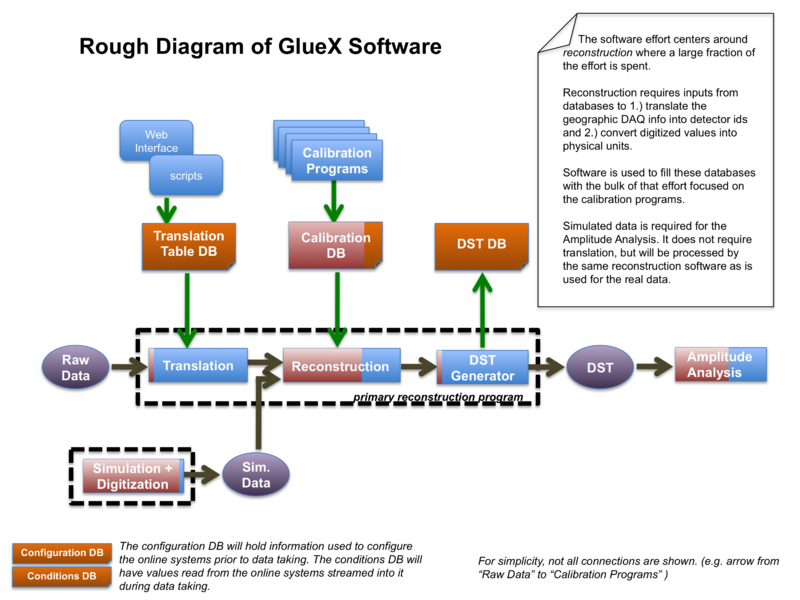
\includegraphics[width=3.5in]{overview_diagram.png}
}

\f{
\ft{Data/Analysis Flow}

\bi
\I Processors
   \bi
   \I Simulation/Digitization
      \bi
      \I GEANT3-based
      \I mature
      \ei
   \I Reconstruction
      \bi
      \I based on Jana framework (multi-threaded)
      \I functional
      \ei
   \I Mini-DST generator
      \bi
      \I planned
      \ei
   \ei
\ei
}
\f{
\ft{Data/Analysis Flow}

\bi
\I Serialized data formats
   \bi
   \I Raw data
      \bi
      \I EVIO: CODA format
      \ei
   \I Simulated data
      \bi
      \I HDDM: Hall D Data Model (XML-like, compressed)
      \ei
   \I Reconstructed data
      \bi
      \I HDDM
      \ei
   \I DST
      \bi
      \I planned
      \ei
   \ei
\ei
}
\f{
\ft{Data/Analysis Flow}

\bi
\I Databases
   \bi
   \I Translation Tables
      \bi
      \I planned
      \ei
   \I Calibrations
      \bi
      \I developed, in beta (Hall B as well)
      \ei
   \I DST
      \bi
      \I planned
      \ei
   \ei
\ei
}

% 2 Manpower Estimates A slide showing the broken out tasks with \%
% complete, manpower needed to complete and names of people with
% institutions that are responsible for the tasks. Conclusion that at
% least at the present, we appear to have sufficient manpower to
% complete the tasks in the time given. 120s (1210s)

\f{
\ft{Manpower: Requirements and Resources}

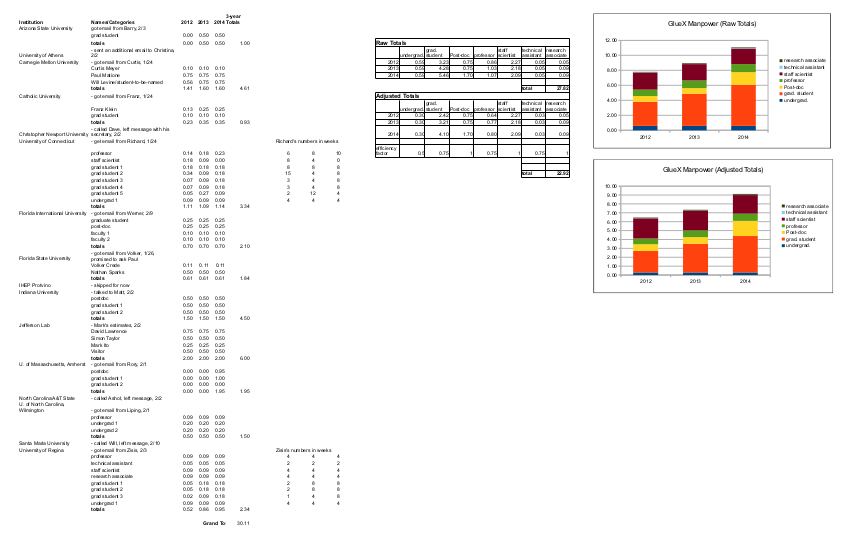
\includegraphics[width=3.5in]{manpower_survey.png}
}
\f{
\ft{Manpower: Requirements and Resources}
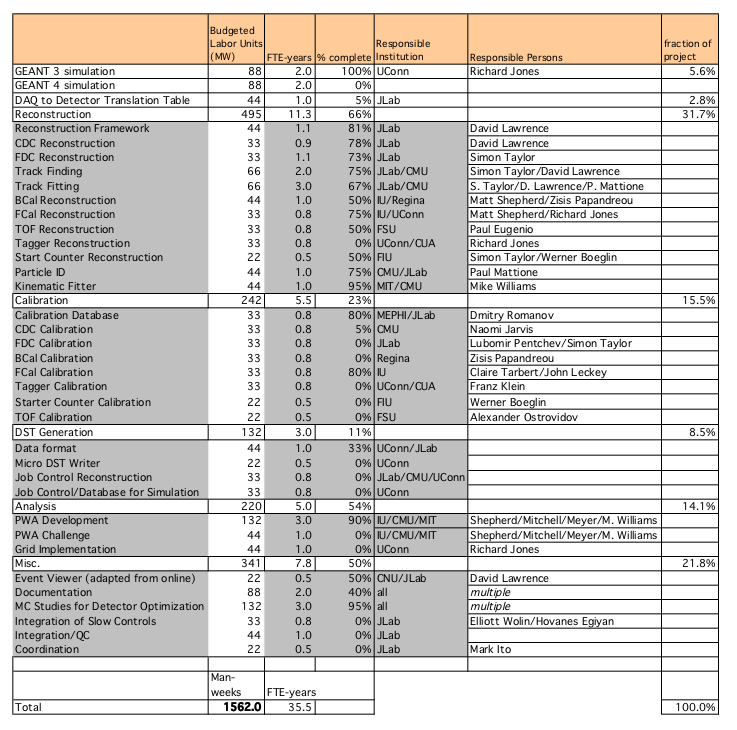
\includegraphics[height=3.0in]{OfflineComputingActivities2012.png}
}

% 3 Software Management A slide showing how the Offline group is
% organized, and how it interacts with the other groups involved in
% related tasks. 60s (1270s)

\f{
\ft{Software Management}
(org chart goes here)
}

% 4 Data/Compute Model A slide based on Mark’s spread sheet showing
% the way that we estimate data volumes and CPU needs. Discuss phase
% I, II and III. 120s (1390s)

\f{
\ft{Data/Compute Model}


Assumptions:
\bi
   \I 20 kHz off detector
   \I 15 kB events
   \I run 35 weeks year, 50\% running efficiency
   \I 130 ms to reconstruct an event (measured)
   \I 5\% of data to calibrate
   \I 2 Monte Carlo events per data event
   \I 67 ms to generate Monte Carlo events (reconstruction time comparable to data)
   \I repetition factor: 2
   \I Other loads:
      \bi
      \I skims/mini-DST production
      \I physics analysis
      \I partial wave analysis
      \ei
\ei

}

\f{\ft{Summary of Requirements}
\bc
\begin{tabular}{|l|r|r|r|}
\hline
Process & CPU (kCores) & Disk (TB) & Tape (PB/y)\\
\hline
Raw Data & -- & -- & 3.2 \\
Calibration & 0.09 & -- & 0.06 \\
Reconstruction & 1.8 & -- & 1.3 \\
Streaming & 0.9 & -- & 0.6 \\
Analysis & 0.9 & 200 & -- \\
Simulation & 5.4 & -- & 2.5 \\
\hline
Total & 9 & 200 & 8 \\
\hline
\end{tabular}
\ec
}

% 5 Calibration/Alignment What needs to be calibrated and how will it
% be done? What has been done already? pi0 calibration of the FCAL,
% CDC prototype alignment and calibration, others? Beam tests? 120s
% (1510s)

\f{
\ft{Calibration/Alignment}
\bi
\I Developing plans for calibration
   \bi
   \I Each working group tasked to list methods, data requirements, compute requirements
   \I Examples:
      \bi
      \I pi0 calibration of forward calorimeter
      \I run plan for tracking chamber alignment
      \I time walk corrections for time-of-flight using plane-to-plane information
      \ei
   \ei
\I Not very advanced on this front; people are busy building detectors
\ei
}

% 6 Data Analysis Model Lay out the model for analysis of GlueX
% data. Raw data on tape/disk at Jefferson Lab. DST’s produced at
% Jefferson Lab, on Tape/Disk. MiniDSTs produced at Jefferson Lab and
% then both analyzed on site and moved off site utilizing
% grid-ftp. 120s (1630s)

\f{
\ft{Data Analysis Model}
   \bi
   \I From detector to CODA EMU's to monitoring farm to online cache disk
   \I Over network to Tape Library in Computer Center
   \I Reconstruction on JLab batch farm, reduction of volume by factor of 10
   \I Reconstructed data written to Tape Library: some fraction live on disk
   \I DST's in several streams produced: large fraction live on disk
   \I Similiar scenario for Monte Carlo except ``raw'' Monte Carlo not kept
   \I Analysis engines access this data:
      \bi
      \I JLab batch farm
      \I Individual work stations
      \I Collaborating institutions
      \I Grid resources
      \I PWA resources
      \ei
   \ei
}

% 7 Simulation Lay out the model for GlueX simulation. Production both
% at Jefferson Lab and at remote sites. Simulation will produce
% MiniDSTs that will need to be moved. All other data is likely
% flushed. What are the expecte resources in outside sites? 120s
% (1760s)

\f{
\ft{Expected Non-JLab Resources}
[survey results go here]
}

% 8 Open Science Grid Discuss that GlueX is a virtual organization in
% the OSG. Some resources from outside are committed to the grid. 120s
% (1890s)

\f{
\ft{Open Science Grid}

\bi
\I Have established GlueX VO with the OSG
\I Nodes from UConn have been contributed
\I Significant analysis has been performed using the grid (3-pi analysis)
\I Grid tools have been installed at JLab (no significant use yet)
\I Plan to use Grid resources to augment those at JLab
   \bi
   \I Monte Carlo generation and reconstruction
   \I Possible to have quick turn-around on specific tasks
   \ei
\ei
}

% 9 Amplitude Analysis On GPUs 60s (1950s)

\f{
\ft{Amplitude Analysis on GPU's}

\bi
\I Calculation of log likelihoods for individual events
   \bi
   \I independent for each events
   \I computationally expensive
   \I not branch intensive
   \I result is small (in bytes)
   \I results are to be summed
   \ei
\I Technique being used by many experiments
\I One of leading implementations developed by GlueX collaborator: AmpTools
\I Large reduction in scale of compute task
\I Infrastructure will evolve
\I Used in 3-pi analysis
\ei
}

% 10 Data Challenge What sort of data challenge do we need? When? 60s
% (2000s)

\f{
\ft{Data Challenges}

\bi
\I Plans only
\I Simulate raw data to DST chain on a large scale
   \bi
   \I Need to develop job management tools
   \ei
\I Establish viability of data transfer capability, to and from JLab
   \bi
   \I Need to establish data management tools (meta-data catalog)
   \ei
\ei
}

\f{
\ft{Reconstruction: Efficiency and Resolution}
\bi
   \I Major area of effort right now
   \I Track reconstruction in a non-uniform magnetic field
      \bi
      \I curling tracks
      \I areas of reduced efficiency/resolution
      \I reconstruction speed
      \ei
   \I Photon reconstruction
      \bi
      \I split-offs
      \I merged clusters
      \I effort to lower thresholds
      \I hadronic contamination
      \ei
\ei
}

% 11 Summary/Conclusion Summarize where we are and where we are
% going. List of what still needs to be done? Contingencies. 60s
% (2060s)

\f{
\ft{Summary/Conclusions}
Accomplishments
\bi
\I End-to-end solution for reconstruction, simlulation, DST-generation in hand
   \bi
   \I neutral and charged particles
   \ei
\I Amplitude analysis capability demonstrated
   \bi
   \I GPU method developed
   \ei
\ei
To Do
\bi
\I Calibration
\I Large-scale data challenges
\I Reconstruction efficiency and resolution
\ei
}

\end{document}
